% !Mode::"TeX:UTF-8"
% !Mode:: "TeX:UTF-8"
\documentclass[xcolor=svgnames,serif,table,10pt]{beamer}
\mode<presentation>{
% Setup appearance:
\useoutertheme{infolines}
\usetheme{Darmstadt}
\setbeamercovered{transparent}
\setbeamertemplate{caption}[numbered]
\setbeamertemplate{navigation symbols}{}
\setbeamertemplate{blocks}[rounded][shadow=true]
\setbeamertemplate{enumerate items}[circle]

% 修改样式
\setbeamercolor{box}{bg=black!20!orange,fg=white}
\setbeamercolor{block title}{use=sidebar,fg=sidebar.fg!10!white,bg=orange!70!black}
\setbeamercolor{block title example}{use=sidebar,fg=sidebar.fg!10!white,bg=black!60!green}
\setbeamercolor{block title alerted}{use=sidebar,fg=sidebar.fg!10!white,bg=black!50!red}

\setbeamertemplate{headline}
{%
  \begin{beamercolorbox}[shadow=true]{section in head/foot}
  \vskip2pt\insertnavigation{\paperwidth}\vskip2pt
  \end{beamercolorbox}%
}
}
\usepackage{url}
\usepackage{animate}
\usepackage[english]{babel}
\usepackage{times}
\usepackage[T1]{fontenc}
\usepackage{multirow,multicol,longtable}
\usepackage{graphics}
\usepackage{xcolor}
\usepackage[no-math]{fontspec}%-------------------------------------------------- 提供字体选择命令
\usepackage{xunicode}%----------------------------------------------------------- 提供Unicode字符宏
\usepackage{xltxtra}%------------------------------------------------------------ 提供了针对XeTeX的改进并且加入了XeTeX的LOGO
\usepackage[BoldFont,SlantFont,CJKchecksingle]{xeCJK}%--------------------------- 使用xeCJK宏包


%================================== 设置中文字体 ================================%
%\setCJKmainfont{Adobe Heiti Std}%------------------------------------------------设置正文为黑体
%\setCJKmonofont{Adobe Song Std}%-------------------------------------------------设置等距字体
%\setCJKsansfont{Adobe Kaiti Std}%------------------------------------------------设置无衬线字体
% \setCJKfamilyfont{zxzt}{FZShouJinShu-S10S}
% \setCJKfamilyfont{FZDH}{FZDaHei-B02S}
%================================== 设置中文字体 ================================%

%================================== 设置英文字体 ================================%
\setmainfont[Mapping=tex-text]{Times New Roman}%--------------------------------英文衬线字体
\setsansfont[Mapping=tex-text]{Arial}%------------------------------------英文无衬线字体
\setmonofont[Mapping=tex-text]{Courier New}%-------------------------------------英文等宽字体
\newfontfamily\Arial{Arial}
%================================== 设置英文字体 ================================%

%================================== 设置数学字体 ================================%
%\setmathsfont(Digits,Latin,Greek)[Numbers={Lining,Proportional}]{Minion Pro}
%================================== 设置数学字体 ================================%
\punctstyle{kaiming}%------------------------------------------------------------ 开明式标点格式
\usepackage{graphicx}
\usepackage{tikz}
\usetikzlibrary{positioning,backgrounds}
\usetikzlibrary{fadings}
\usetikzlibrary{patterns}
\usetikzlibrary{calc}
\usetikzlibrary{shadings}
\pgfdeclarelayer{background}
\pgfdeclarelayer{foreground}
\pgfsetlayers{background,main,foreground}
\usepackage{xifthen}
\usepackage{colortbl,dcolumn}
\usepackage{enumerate}
\usepackage{pifont}
\usepackage{tabularx}
\usepackage{booktabs}
\usepackage{hyperref}

\usepackage{bm} % 字体加粗的方法
\usetikzlibrary{arrows,automata,matrix,arrows}

%=================================== 数学符号 =================================%
\newcommand{\rtn}{\mathrm{\mathbf{R}}}
\newcommand{\N}{\mathrm{\mathbf{N}}}
\newcommand{\As}{\mathrm{a.s.}}
\newcommand{\Ae}{\mathrm{a.e.}}
\newcommand*{\PR}{\mathrm{\mathbf{P}}}
\newcommand*{\EX}{\mathrm{\mathbf{E}}}
\newcommand{\EXlr}[1]{\mathrm{\mathbf{E}}\left[#1\right]}
\newcommand*{\dif}{\,\mathrm{d}}
\newcommand*{\F}{\mathcal{F}}
\newcommand*{\h}{\mathcal{H}}
\newcommand*{\vp}{\varepsilon}
\newcommand*{\prs}{\dif\PR-\As}
\newcommand*{\dte}{\dif t-\Ae}
\newcommand*{\pts}{\dif\PR\times\dif t-\Ae}
\newcommand{\Ito}{It\^{o}}
\newcommand{\tT}[1][0]{[#1,T]}
\newcommand{\intT}[2][T]{\int^{#1}_{#2}}
\newcommand{\intTe}[1][t]{\intT[t+\varepsilon]{#1}}
\newcommand{\s}{\mathcal{S}}
\newcommand{\me}{\mathrm{e}}
\newcommand{\one}[1]{{\bf 1}_{#1}}
\renewcommand{\M}{{\rm M}}
\newcommand{\Me}[1][t]{M^{\varepsilon}_{#1}}
\newcommand{\Ne}[1][t]{N^{\varepsilon}_{#1}}
\newcommand{\Pe}[1][t]{P^{\varepsilon}_{#1}}
\DeclareMathOperator*{\sgn}{sgn}
% =================================== 数学符号 =================================%

% 定义罗马数字
\makeatletter
\newcommand{\rmnum}[1]{\romannumeral #1}
\newcommand{\Rmnum}[1]{\expandafter\@slowromancap\romannumeral #1@}
\makeatother

% 定义破折号
\newcommand{\pozhehao}{\kern0.3ex\rule[0.8ex]{2em}{0.1ex}\kern0.3ex}
% 中文日期
\def\CJK@today{\the\year 年 \the\month 月}
\newcommand\zhtoday{\CJK@today}

% 中文图表
\renewcommand\figurename{图}
\renewcommand\tablename{表}

\usepackage{verbatim} % \begin{comment} xxxx \end{comment}

\usetheme{Berlin} %主题
%\usecolortheme{sustech} %主题颜色

\usepackage{algorithm}  
\usepackage{algorithmicx}  
\usepackage{algpseudocode}
\floatname{algorithm}{算法}
\renewcommand{\algorithmicrequire}{\textbf{输入:}} 
\renewcommand{\algorithmicensure}{\textbf{输出:}}  

\algrenewcommand{\algorithmiccomment}[1]{ $//$ #1}

\definecolor{mygreen}{rgb}{0,0.6,0}
\definecolor{mygray}{rgb}{0.5,0.5,0.5}
\definecolor{mymauve}{rgb}{0.58,0,0.82}
\usepackage{listings}
\lstset{ %
	backgroundcolor=\color{white},   % choose the background color
	basicstyle=\footnotesize\ttfamily,     % size of fonts used for the code
	columns=fullflexible,
	breaklines=true,                 % automatic line breaking only at whitespace
	captionpos=b,                    % sets the caption-position to bottom
	tabsize=4,
	commentstyle=\color{mygreen},    % comment style
	escapeinside={\%*}{*)},          % if you want to add LaTeX within your code
	keywordstyle=\color{blue},       % keyword style
	stringstyle=\color{mymauve}\ttfamily,     % string literal style
	numbers=left, 
	%	frame=single,
	rulesepcolor=\color{red!20!green!20!blue!20},
	% identifierstyle=\color{red},
	language=c
}

\graphicspath{{figures/},} 

% Author, Title, etc.

\title{计算机导论与程序设计[CS006001-60]}

%% \subtitle{Foreground-constrained Eulerian Video Motion Magnification}

\author[段江涛]{段江涛
\\机电工程学院}

\institute[]{
\includegraphics[height=1cm]{xd.jpg}}

\date{\zhtoday}

\setlength{\baselineskip}{22pt}
\renewcommand{\baselinestretch}{1.4}

% The main document

\begin{document}
\setlength{\abovedisplayskip}{1ex}%------------------------------------------ 公式前的距离
\setlength{\belowdisplayskip}{1ex}%------------------------------------------ 公式后的距离

\begin{frame}
  \titlepage
\end{frame}

%%%%%%%%%%%%%%%%%%%%%%%%%%%%%%%%
%%%%%%%%%%%%%%%%%%%%%%%%%%%%%%%%
%%%%%%%%%%%%%%%%%%%%%%%%%%% lecture-1
\begin{frame}
  \frametitle{lecture-1 主要内容}
  \tableofcontents[hideallsubsections]
\end{frame}

\section{课程介绍}

\begin{frame}{课程内容}
\begin{itemize}
	\item 计算机导论:了解计算机的基本知识;掌握计算机操作基本技能。
	\item 程序设计:掌握结构化程序设计方法。会读、会编、会调试C语言程序。
	\item 教材
	\begin{itemize}
		\item 大学计算机,龚尚福, 贾澎涛,西安电子科技大学出版社
		\item C程序设计第五版, 谭浩强,清华大学出版社
	\end{itemize}
\end{itemize}
\end{frame}

\begin{frame}{考核}
\begin{enumerate}
	\item 导论部分计算机应用成绩(C1): 10\%。计算机基本操作技能。
	\item 导论部分课程报告成绩(C2): 10\%。撰写课程学习小论文。
	\item 单元测验成绩(C3、C4): 40\%。根据机试系统给出的练习题目编写程序,通过调试得到正确结果并通过\textbf{机试系统提交}。
	\item 平时作业成绩(C5): 10\%。主要考核对每堂课知识点的复习、理解和掌握程度。
	\item 期末考试成绩(C6): 30\%。主要考程序设计思想、逻辑思维、程序设计方法、程序调试能力。\textbf{考试形式为机试}。
\end{enumerate}
\end{frame}

\section{导论简介}

\begin{frame}{计算机导论主要内容}
\textbf{总体要求: 了解计算机的基本知识; 掌握计算机操作基本技能。}\\
\begin{itemize}
	\item 计算机系统组成
	\item 计算机工作原理
	\item 操作系统
	\item 字处理: Microsoft Word
	\item 电子表格: Microsoft Excel
	\item 演示文稿: Microsoft PowerPoint
\end{itemize}
\end{frame}

\begin{frame}{计算机工作原理}
\textbf{工作原理: ``存储程序'' + ``程序控制''}
\begin{enumerate}
	\item 以\textbf{二进制}形式表示数据和指令
	\item 将程序存入存储器中,由控制器自动读取并执行
	\item 外部存储器存储的程序和所需数据$\implies$计算机内存$\implies$在程序控制下由CPU周而复始地取出指令、分析指令、执行指令$\implies$操作完成。	
\end{enumerate}
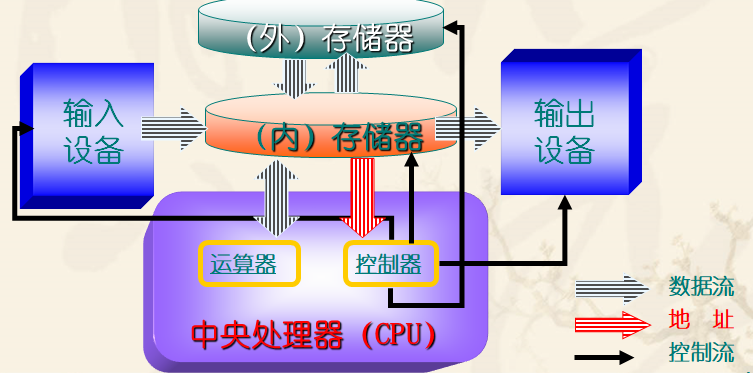
\includegraphics[scale=0.25]{hframe}
\end{frame}

\begin{frame}[shrink]
\frametitle{10进制,2进制,16进制的幂展开式}
\begin{align*}
(D)_{10}&=D_{n-1}\times 10^{n-1}+D_{n-2}\times 10^{n-2}+\cdots+D_{1}\times 10^{1}+D_{0}\times 10^{0}\\
&+D_{-1}\times 10^{-1}+D_{-2}\times 10^{-2}+\cdots+D_{-m+1}\times 10^{-m+1}+D_{-m}\times 10^{-m}\\
(B)_{2}&=B_{n-1}\times 2^{n-1}+B_{n-2}\times 2^{n-2}+\cdots+B_{1}\times 2^{1}+B_{0}\times 2^{0}\\
&+B_{-1}\times 2^{-1}+B_{-2}\times 2^{-2}+\cdots+B_{-m+1}\times 2^{-m+1}+B_{-m}\times 2^{-m}\\
(H)_{2}&=H_{n-1}\times 16^{n-1}+H_{n-2}\times 16^{n-2}+\cdots+H_{1}\times 16^{1}+H_{0}\times 16^{0}\\
&+H_{-1}\times 16^{-1}+H_{-2}\times 16^{-2}+\cdots+16_{-m+1}\times 16^{-m+1}+H_{-m}\times 16^{-m}
\end{align*}
\end{frame}

\begin{frame}{进制对照表}
\begin{tabular}{|c|c||c|c|}
	\hline 
	二进制 & 十六进制 & 二进制 & 十六进制 \\ 
	\hline 
	0000 &  0 & 1000  & 8 \\ 
	\hline 
	0001 &  1 & 1001  & 9 \\ 
	\hline 
	0010 &  2 & 1010  & A \\ 
	\hline 
	0011 &  3 & 1011  & B \\ 
	\hline 
	0100 &  4 & 1100  & C \\ 
	\hline 
	0101 &  5 & 1101  & D \\ 
	\hline 
	0110 &  6 & 1110  & E \\ 
	\hline 
	0111 &  7 & 1111  & F \\ 
	\hline 
\end{tabular} 
\end{frame}

\begin{frame}
\begin{example}
	\begin{align*}
	(123)_{10}&=1\times 10^2+2\times 10^1+3\times 10^0; \\
	&3=123\%10, 2=123/10\%10, 1=123/10/10\%10\\
	\newline
	(77)_{10}&=(0100\quad 1101)_{2}=0\times 2^7+1\times 2^6+0\times 2^5+0\times 2^4\\
	&+1\times 2^3+1\times 2^2+0\times 2^1+1\times 2^0\\
	\newline
	(77)_{10}&=(4D)_{16}=4\times 16^1+13\times 16^0
	\end{align*}
\end{example}
\end{frame}

\begin{frame}{数值在计算机中的表示(以8bit编码为例)}
\begin{itemize}
	\item 原码:正数的符号为0,负数的符号为1,其它位按一般的方法表示数的绝对值。
	\begin{align*}
	x=(+103)_{10}  &&[x]_{\text{原}}=(01100111)_{2}\\
	x=(-103)_{10}  &&[x]_{\text{原}}=(11100111)_{2}
	\end{align*}
	\item 反码: 正数的反码与原码相同;负数的反码是符号位不变,其他位按位取反 
	\item 补码: 正数的补码与其原码相同;负数的补码为其反码最末位加1. 即, \textcolor{blue}{补码 = 反码+1}
\end{itemize}
\begin{align*}
(77)_{10}&=(0100\quad 1101)_{2},\qquad (-77)_{10}=(1100\quad 1101)_{2}\\
(-77)_{\text{补}}=2^8-77&=1111\quad 1111 - 0100\quad 1101 +0000\quad 0001\\
	&=1011\quad 0010 + 0000\quad 0001=1011\quad 0011
\end{align*}
\end{frame}

\begin{frame}{机内以补码形式存储有符号数}
\begin{enumerate}
	\item 对于正数,原码=反码=补码
	\item 对于负数,补码=反码 + 1\\
	      反码 = 符号位不变, 其他位按位取反
	\item 补码是可逆的,即再对补码求补得到原码。
	\item 引入补码后,使减法统一为加法。	
\end{enumerate}
\end{frame}

\begin{frame}{数值表示示例}
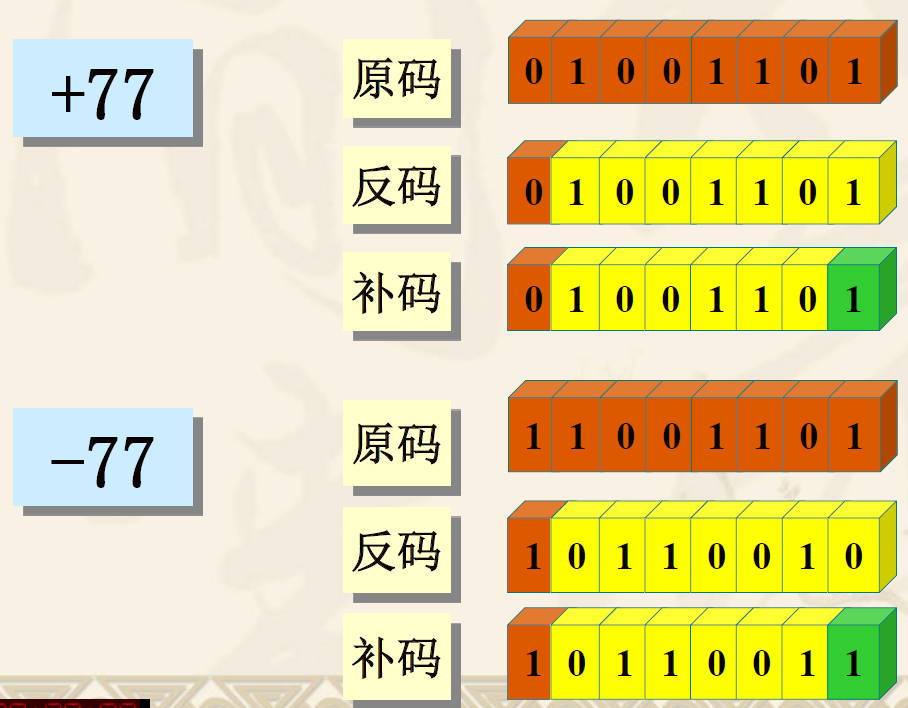
\includegraphics[scale=0.25]{2}
\end{frame}

\begin{frame}{ASCII编码表$B_6B_5B_4B_3B_2B_1B_0$}
\begin{columns}
	\column{0.7\textwidth}
	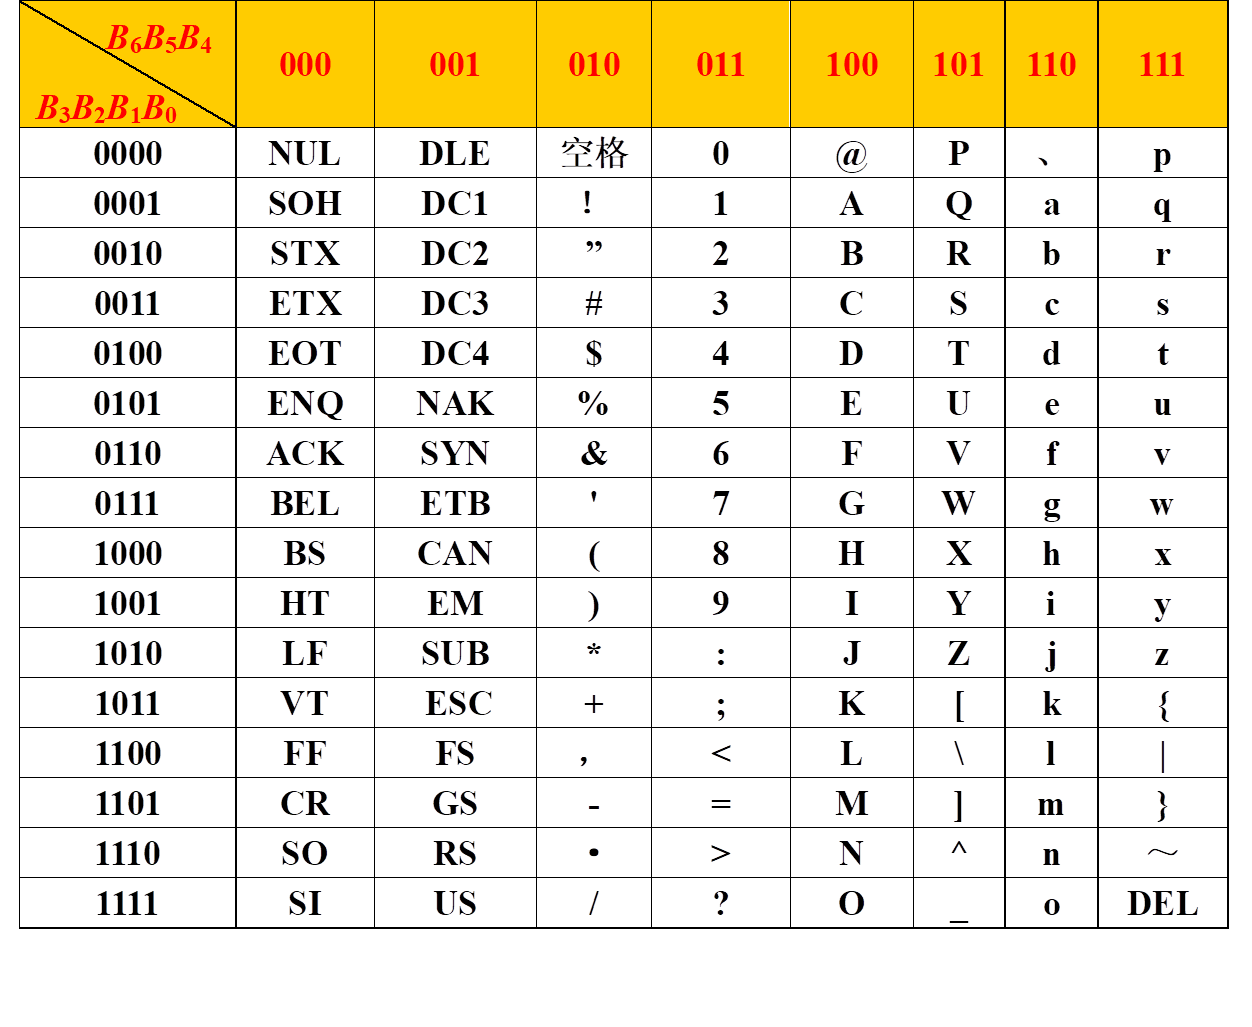
\includegraphics[scale=0.4]{ASCII}
	\column{0.3\textwidth}
	\begin{itemize}
		\item ASCII码连续排列 \\
		 `0'$\sim$`9', `A'$\sim$`Z', `a'$\sim$`z'
		\item 数字 = 编码值 - `0' \\
		 9=`9'-`0'
		\item 大小字符间隔: \\
		`a' - `A' = 32
	\end{itemize}	
\end{columns}
\end{frame}

\section{C语言程序设计}

\begin{frame}{计算机程序}

\includegraphics[scale=0.4]{program1}
\end{frame}

\begin{frame}{计算机语言}
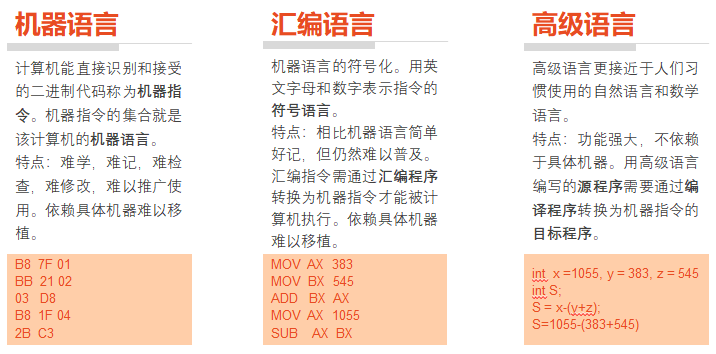
\includegraphics[scale=0.4]{program2}
\end{frame}

\begin{frame}{高级语言的发展}

\includegraphics[scale=0.4]{program3}
\end{frame}

\begin{frame}{C语言的特点}
\begin{enumerate}
	\item 语言简洁、紧凑,使用方便、灵活
    \item 运算符丰富
    \item 数据类型丰富
    \item \textcolor{blue}{C语言是完全模块化和结构化的语言}\\
          具有结构化的控制语句(顺序、选择、循环结构)\\
          用函数作为程序的模块单位,便于实现程序的模块化
    \item \textcolor{blue}{兼具高级语言和低级语言的功能}\\
          允许直接访问物理地址\\
          能进行位(bit)操作\\  
          能实现汇编语言的大部分功能\\
          可以直接对硬件进行操作        
\end{enumerate}
\end{frame}

\begin{frame}{程序设计的任务}
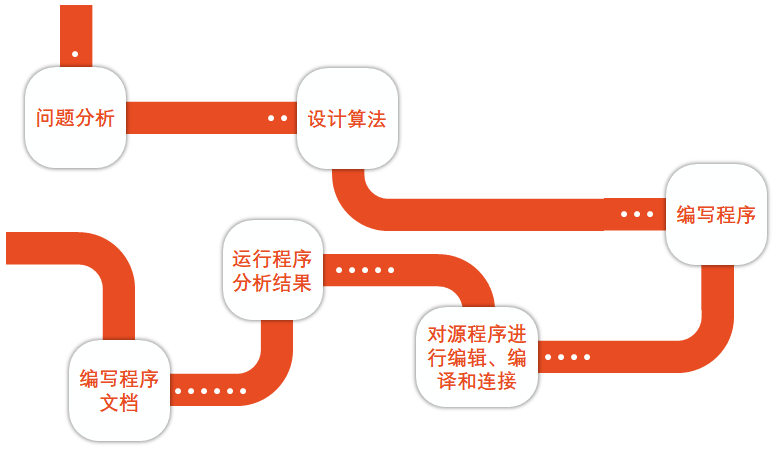
\includegraphics[scale=0.4]{program}
\end{frame}

\begin{frame}[fragile]{第一个C语言程序}
    \begin{lstlisting}
    #include<stdio.h>            // standard input/output编译预处理指令
    int main()                   // 主函数
    {                            // 函数开始标志
       printf("Hello World!");   // 输出一行信息
       return 0;                 // 函数执行完毕返回函数值0
    }                            // 函数结束标志
    \end{lstlisting}
\end{frame}

\begin{frame}[fragile]{求两个整数之和}
\begin{lstlisting}
#include<stdio.h>            // standard input/output编译预处理指令
int main()                   // 主函数
{                            // 函数开始标志
   int a,b,sum;           // 定义a,b,sum为整型变量
   a=123;                 // 对a,b赋值
   b=456;
   sum=a+b;              // 计算a+b, 并把结果存放在变量sum中
   printf("sum is %d\n",sum);   // 输出结果
   return 0;                 // 函数执行完毕返回函数值0
}                            // 函数结束标志
\end{lstlisting}
\end{frame}

\begin{frame}{运行C程序的步骤与方法}
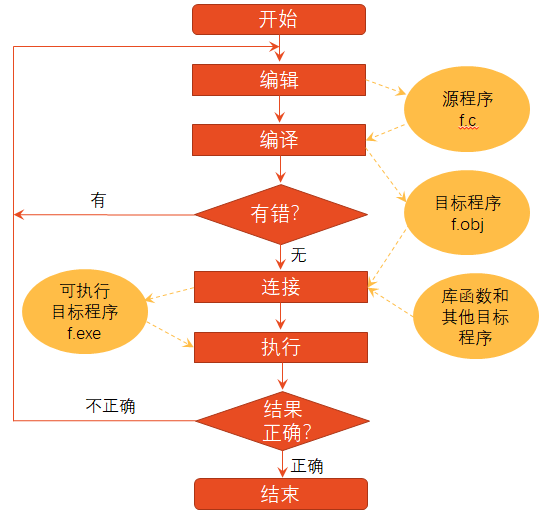
\includegraphics[scale=0.45]{program4}
\end{frame}

\begin{frame}{集成开发环境---编译系统}
\begin{itemize}
	\item Bloodshed Dev-C++ 
	\item Turbo C
	\item Visual C++6.0 
	\item Visual Studio(VS2015,VS Community 2019等)
\end{itemize}
\end{frame}

\begin{frame}{Bloodshed Dev-C++集成开发环境}
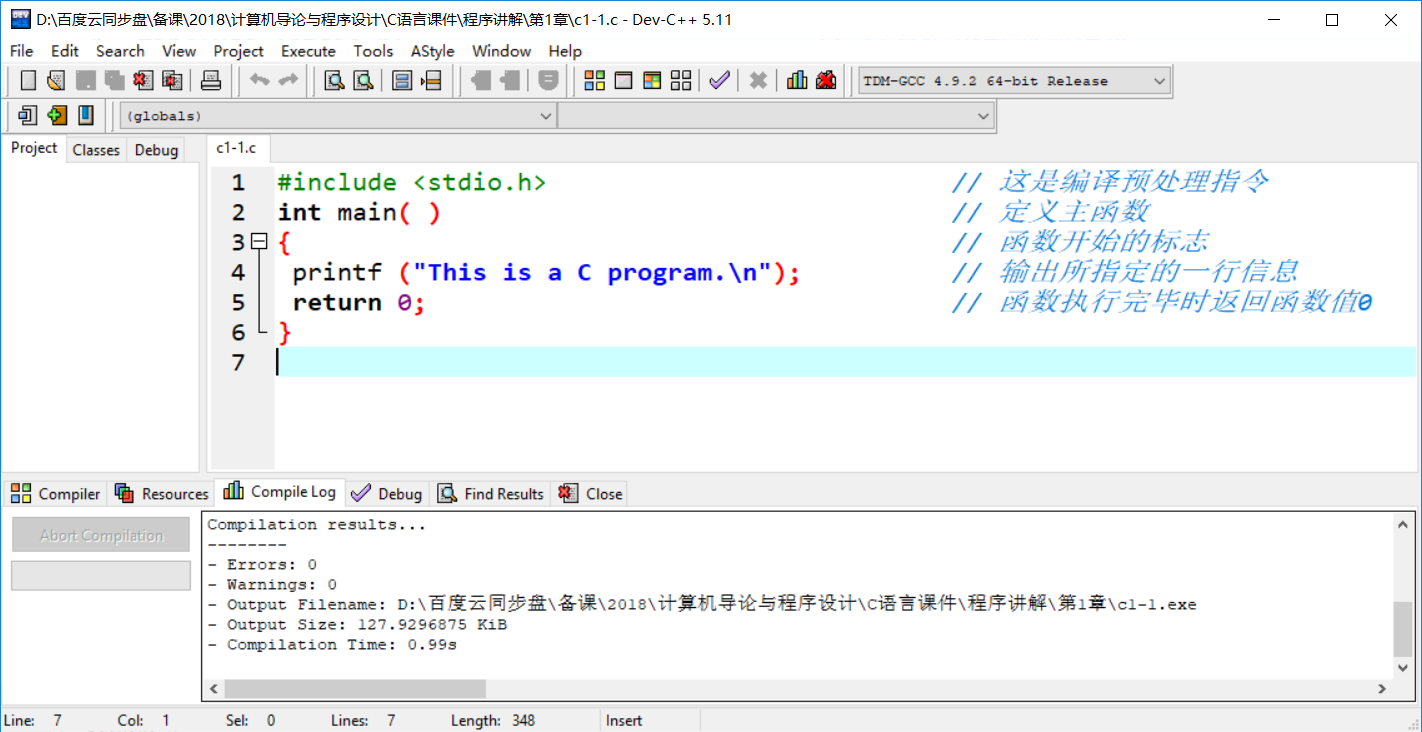
\includegraphics[scale=0.3]{DevCpp}   
\end{frame}

\begin{frame}{Bloodshed Dev-C++集成开发环境}
\begin{itemize}
	\item 选择“文件”菜单,选择“源文件”, 编辑程序。
	\item 保存时,保存为 .cpp或 .c文件。
	\item 选择“编译和运行”菜单,生成.exe文件,运行程序。  
\end{itemize} 
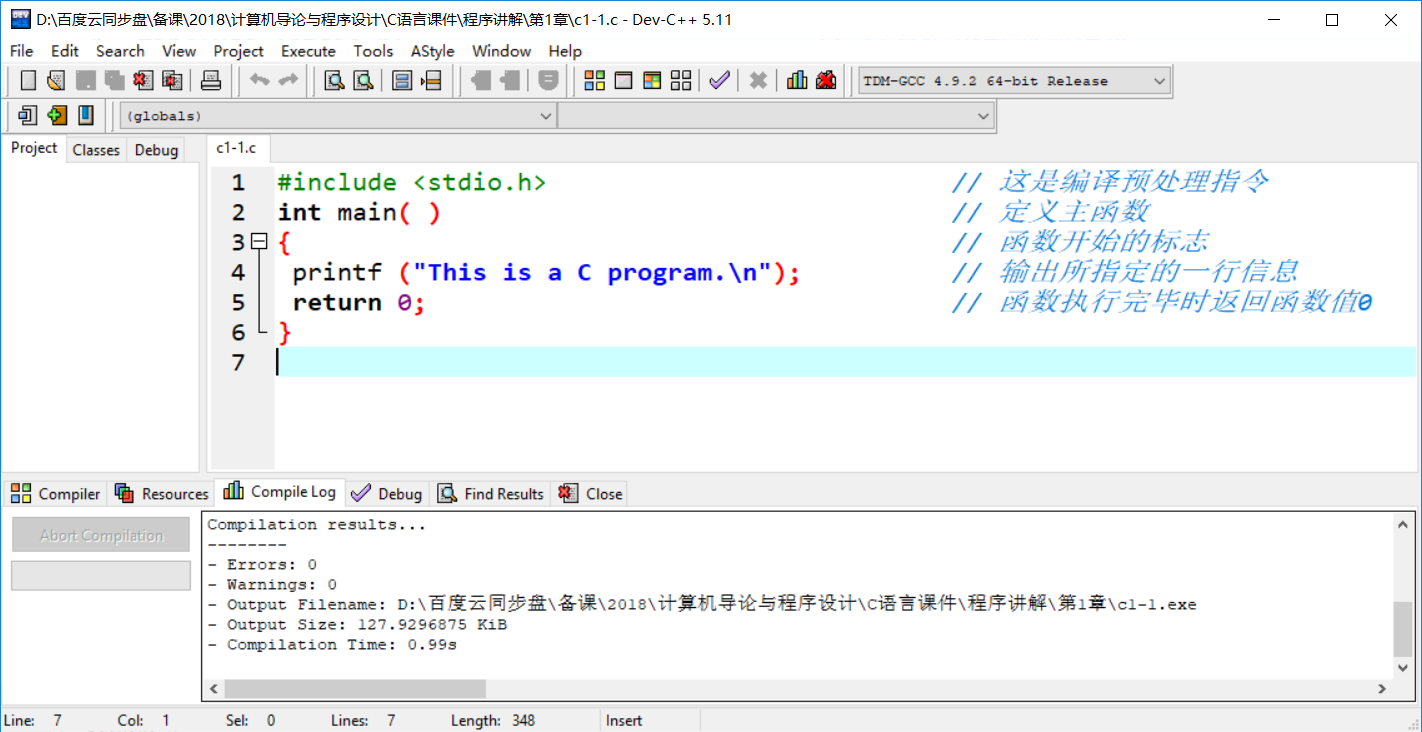
\includegraphics[scale=0.2]{DevCpp}   
\end{frame}
%%%%%%%%%%%%%%%%%%%%%%%%%% lecture-2
%\begin{frame}
%  \frametitle{lecture-2 算法---程序的灵魂}
%  \tableofcontents[hideallsubsections]
%\end{frame}

\section{数据类型}

\begin{frame}{基本数据类型}
\begin{itemize}
	\item 整数\lstinline|int|
	\item 单精度浮点数\lstinline|float|
	\item 双精度浮点数\lstinline|double|
	\item 字符\lstinline|char|
\end{itemize}
\textcolor{red}{机内用二进制表示, 不同数据类型占用存储空间大小不同。}
\end{frame}

\begin{frame}[fragile]{变量在使用之前首先要定义它的数据类型}
\begin{lstlisting}
#include<stdio.h>            // standard input/output编译预处理指令
int main()                   // 主函数
{                            // 函数开始标志
	int a,b;  // 定义变量a, b为整型数值,同类型变量可以在一条语句中定义。
	float f;  // 定义变量f为单精度浮点数
	double d; // 定义变量d为双精度浮点数
	char c;   // 定义变量c为单个英文字母
	a=10;	  // 变量赋值
	b=20;
	f=10.2;
	d=20.3;
	c='A';	  // 字符用单引号括起来
	return 0;                // 函数执行完毕返回函数值0
}                            // 函数结束标志
\end{lstlisting}
\end{frame}

\begin{frame}[fragile]{标识符}
标识符就是一个对象的名字。用于标识变量、符号常量、函数、数组、类型等。\\
\textcolor{blue}{以字母或下划线开始; 区分大小写; 不能使用关键字; 最好有含义。}
\begin{lstlisting}
#include<stdio.h>           
int main()                   
{                            
	int r = 123; // 合法整型变量名
	int 3a; // 不合法的变量名
	int break; // 不合法的变量名, 因为break是关键字, 被系统使用。
	int Radius; // 变量名最好有含义
	int radius; // 与Radius是不同的变量,C语言是大小写敏感的语言
	return 0;           
}                            
\end{lstlisting}
\end{frame}

\begin{frame}{C语言关键字}
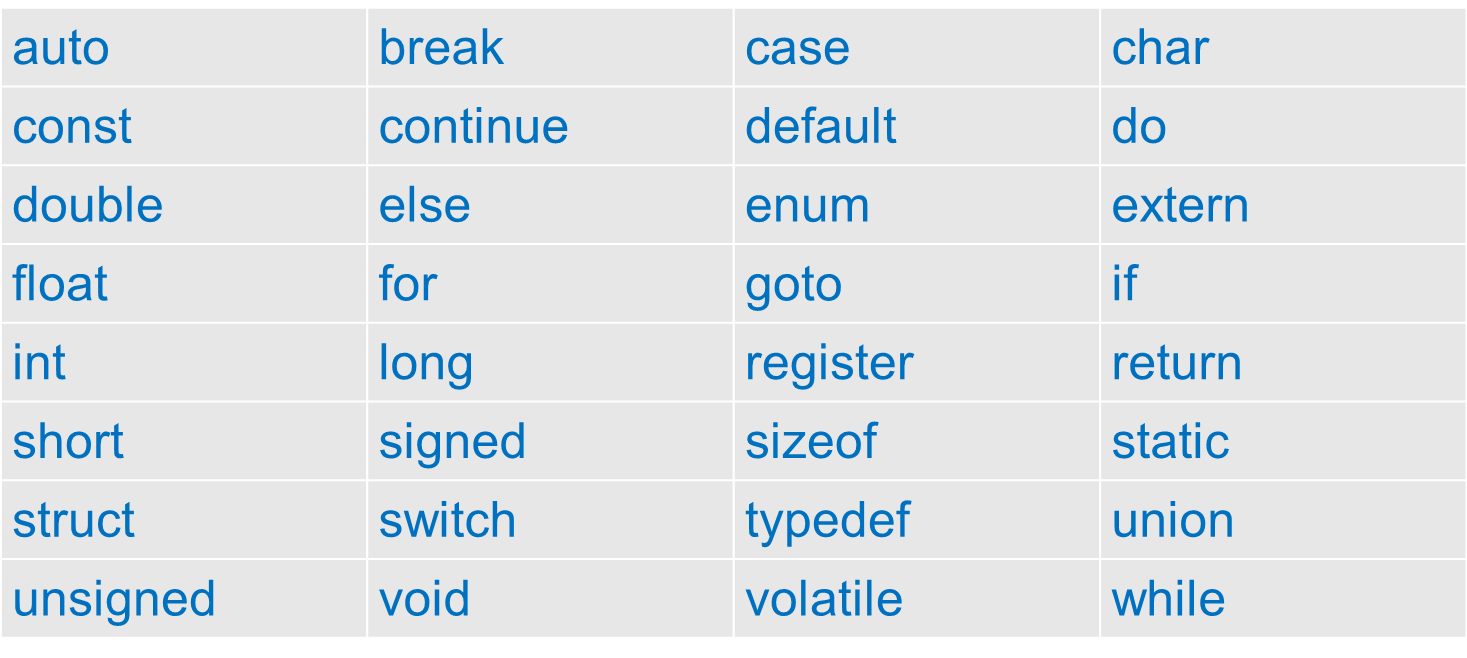
\includegraphics[scale=0.5]{key}
\end{frame}

\begin{frame}[shrink,fragile]{输出语句printf(``原样输出, \%格式符'', 对应变量值);}
\begin{lstlisting}
#include<stdio.h>            // standard input/output编译预处理指令
int main()                   // 主函数
{                            // 函数开始标志
	int a=10,b;    // 定义变量a, b为整型数值, 定义变量时,可以指定变量的初值
	float f=10.2;  // 定义变量f为单精度浮点数
	double d; // 定义变量d为双精度浮点数
	char c;   // 定义变量c为单个英文字母
	f=10.2;
	d=20.356;
	c='A';
	printf("a=%d,b=%d,c=%c,f=%f,d=%.2lf\n",a,b,c,f,d); // %.2f, %.2lf保留两位小数, \n为换行符
	return 0;                // 函数执行完毕返回函数值0
}                            // 函数结束标志
\end{lstlisting}
\textcolor{blue}{变量b没有被赋值, 将是一个随机值。}
\end{frame}

\begin{frame}{常用格式描述符与数据类型的对应关系}
\centering
\begin{tabular}{|c|c|c|}
	\hline 
	\textbf{格式符} & \textbf{对应的数据类型} &  \textbf{备注}\\ 
	\hline 
	\%d & int &  \\ 
	\hline  
	\%f & float &  \\
	\hline
	\%c & char & \\ 
	\hline   
	\%lf & double & \\ 
	\hline 
	\%.2f & float & 保留两位小数, 四舍五入。不适用于scanf()。 \\ 
	\hline 
	\%.2lf & double & 保留两位小数, 四舍五入。不适用于scanf()。 \\ 
	\hline   
	\%x(\%X) & int,char & 十六进制显示(大写) \\ 
	\hline 
	\%ld & long int &  \\ 
	\hline 
\end{tabular}
\newline
\newline
\textcolor{blue}{详见p73, 表3.6}
\end{frame}


\begin{frame}{十进制与二进制}
\vspace{-1cm}
\begin{align*}
&\textcolor{red}{\text{十进制: 以10为底的幂展开式:}}\\
&(123)_{10}=1\times 10^2+2\times 10^1+3\times 10^0; \\
&\textcolor{blue}{\text{自低到高各位数(除10取余至商为0): }3=123\%10,~2=123/10\%10=12\%10,}\\
&\textcolor{blue}{1=123/10/10\%10=1\%10}\\
&\textcolor{red}{\text{二进制: 以2为底的幂展开式:}}\\
&(77)_{10}=(0100\quad 1101)_{2}=0\times 2^7+1\times 2^6+0\times 2^5+0\times 2^4\\
&\qquad +1\times 2^3+1\times 2^2+0\times 2^1+1\times 2^0\\
&\textcolor{blue}{\text{自低到高各位数(除2取余至商为0): }1=77\%2,~0=77/2\%2=38\%2,}\\
&\textcolor{blue}{~1=77/2/2\%2=19\%2,~1=77/2/2/2\%2=9\%2,}\\
&~\textcolor{blue}{0=77/2/2/2/2/\%2=4\%2,~0=77/2/2/2/2/2/\%2=2\%2,\dots}\\
\end{align*}
\end{frame}

\begin{frame}[shrink]
\frametitle{10进制、2进制、16进制的幂展开式}
\vspace{-0.5cm}
\begin{align*}
(D)_{10}&=D_{n-1}\times 10^{n-1}+D_{n-2}\times 10^{n-2}+\cdots+D_{1}\times 10^{1}+D_{0}\times 10^{0}\\
&+D_{-1}\times 10^{-1}+D_{-2}\times 10^{-2}+\cdots+D_{-m+1}\times 10^{-m+1}+D_{-m}\times 10^{-m}\\
&\\
(B)_{2}&=B_{n-1}\times 2^{n-1}+B_{n-2}\times 2^{n-2}+\cdots+B_{1}\times 2^{1}+B_{0}\times 2^{0}\\
&+B_{-1}\times 2^{-1}+B_{-2}\times 2^{-2}+\cdots+B_{-m+1}\times 2^{-m+1}+B_{-m}\times 2^{-m}\\
&\\
(H)_{16}&=H_{n-1}\times 16^{n-1}+H_{n-2}\times 16^{n-2}+\cdots+H_{1}\times 16^{1}+H_{0}\times 16^{0}\\
&+H_{-1}\times 16^{-1}+H_{-2}\times 16^{-2}+\cdots+16_{-m+1}\times 16^{-m+1}+H_{-m}\times 16^{-m}
\end{align*}
\end{frame}

\begin{frame}{进制对照表$2^32^22^12^0=8+4+2+1$}
\centering
\begin{tabular}{|>{\columncolor{yellow}}c|c|c||>{\columncolor{yellow}}c|c|c|}
\hline 
十进制 & 二进制 & 十六进制 & 十进制 & 二进制 & 十六进制 \\ 
\hline 
0 & 0000 &  0 & 8 & 1000  & 8 \\ 
\hline 
1 & 0001 &  1 & 9 & 1001  & 9 \\ 
\hline 
2 & 0010 &  2 & 10 & 1010  & A \\ 
\hline 
3 & 0011 &  3 & 11 & 1011  & B \\ 
\hline 
4 & 0100 &  4 & 12 & 1100  & C \\ 
\hline 
5 & 0101 &  5 & 13 & 1101  & D \\ 
\hline 
6 & 0110 &  6 & 14 & 1110  & E \\ 
\hline 
7 & 0111 &  7 & 15 & 1111  & F \\ 
\hline 
\end{tabular} 
\end{frame}

\begin{frame}{十进制、二进制与十六进制数值分解举例}
\vspace{-0.5cm}
\begin{align*}
(123)_{10}&=1\times 10^2+2\times 10^1+3\times 10^0; \\
&\textcolor{blue}{\text{自低到高各位数: }3=123\%10,~2=123/10\%10,~1=123/10/10\%10}\\
&\\
(77)_{10}&=(0100\quad 1101)_{2}=0\times 2^7+1\times 2^6+0\times 2^5+0\times 2^4\\
&+1\times 2^3+1\times 2^2+0\times 2^1+1\times 2^0\\
&\\
(77)_{10}&=(4D)_{16}=4\times 16^1+13\times 16^0
\end{align*}
\end{frame}

%\begin{frame}[shrink]{数值在计算机中的表示(以8bit编码为例)}
%\begin{itemize}
%	\item 原码:正数的符号为0,负数的符号为1,其它位按一般的方法表示数的绝对值。
%	\vspace{-0.5cm}
%	\begin{align*}
%	x=(+103)_{10}  &&[x]_{\text{原}}=(\textcolor{red}{0}1100111)_{2}\\
%	x=(-103)_{10}  &&[x]_{\text{原}}=(\textcolor{red}{1}1100111)_{2}
%	\end{align*}
%	\item 反码: 正数的反码与原码相同;负数的反码是符号位不变,其他位按位取反 
%	\item 补码: 正数的补码与其原码相同;负数的补码为其反码最末位加1. 即,
%	
%	\textcolor{blue}{负数补码 = 反码$+1=2^n-$该数的绝对值, $n$是编码二进制位数.}
%\end{itemize}
%\vspace{-0.5cm}
%\begin{align*}
%(77)_{10}&=(\textcolor{red}{0}100\quad 1101)_{2},\qquad (-77)_{10}=(\textcolor{red}{1}100\quad 1101)_{2}\\
%(-77)_{\text{补}}=2^8-77&=\textcolor{red}{1}111\quad 1111 +\textcolor{red}{0}000\quad 0001 - \textcolor{red}{0}100\quad 1101\\
%&=\underbrace{\textcolor{red}{1}111\quad 1111 - \textcolor{red}{0}100\quad 1101}_{(-77)_{\text{反}}} + ~\textcolor{red}{0}000\quad 0001\\
%&=\underbrace{\textcolor{red}{1}011\quad 0010 }_{(-77)_{\text{反}}}+ \textcolor{red}{0}000\quad 0001=1011\quad 0011
%\end{align*}
%\end{frame}

\begin{frame}[shrink]{数值在计算机中的表示(以8bit编码为例)}
\begin{tikzpicture}
\node[text width=1\textwidth] (t) {
\begin{itemize}
	\item 原码:正数的符号为0,负数的符号为1,其它位按一般的方法表示数的绝对值。
	\vspace{-0.5cm}
	\begin{align*}
	x=(+103)_{10}  &&[x]_{\text{原}}=(\textcolor{red}{0}1100111)_{2}\\
	x=(-103)_{10}  &&[x]_{\text{原}}=(\textcolor{red}{1}1100111)_{2}
	\end{align*}
	\item 反码: 正数的反码与原码相同;负数的反码是符号位不变,其他位按位取反 
	\item 补码: 正数的补码与其原码相同;负数的补码为其反码最末位加1. 即,
	
	\textcolor{blue}{负数补码 = 反码$+1=2^n-$该数的绝对值, $n$是编码二进制位数.}
\end{itemize}
\vspace{-0.5cm}
\begin{align*}
(77)_{10}&=(\textcolor{red}{0}100\quad 1101)_{2},\qquad (-77)_{10}=(\textcolor{red}{1}100\quad 1101)_{2}\\
(-77)_{\text{补}}=2^8-77&=\textcolor{red}{1}111\quad 1111 +\textcolor{red}{0}000\quad 0001 - \textcolor{red}{0}100\quad 1101\\
&=\underbrace{\textcolor{red}{1}111\quad 1111 - \textcolor{red}{0}100\quad 1101}_{(-77)_{\text{反}}} + ~\textcolor{red}{0}000\quad 0001\\
&=\underbrace{\textcolor{red}{1}011\quad 0010 }_{(-77)_{\text{反}}}+ \textcolor{red}{0}000\quad 0001=1011\quad 0011
\end{align*}
};
\node[anchor=south west,text width=.4\textwidth] at($(t.south west)+(0.2cm,0.2cm)$) {
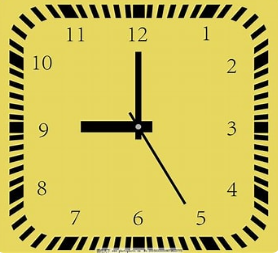
\includegraphics[scale=0.2]{clock}
};
\end{tikzpicture}
\end{frame}

\begin{frame}{数值表示示例}
\centering
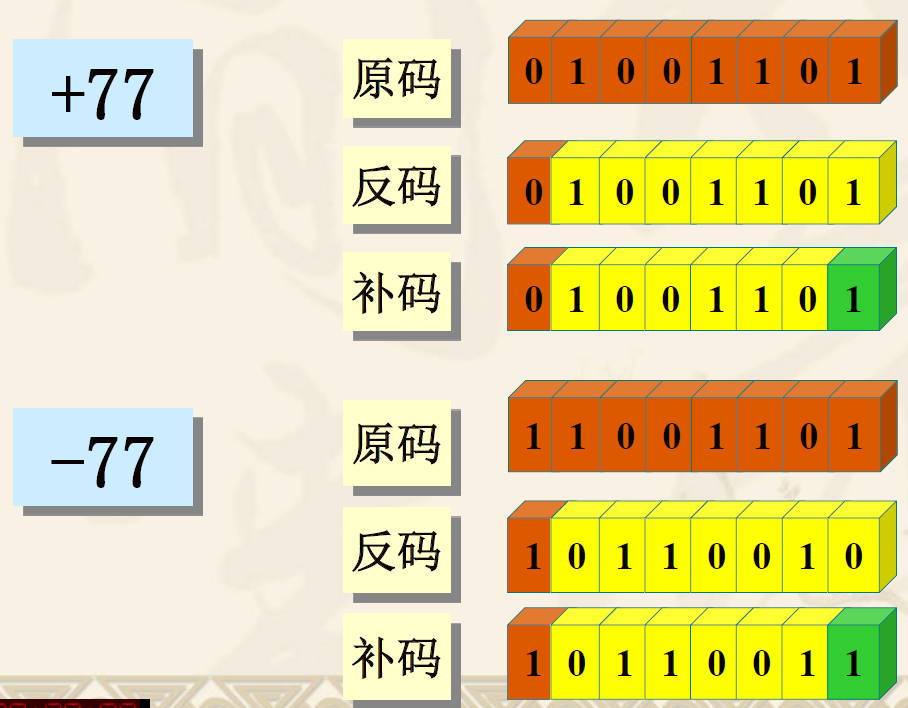
\includegraphics[scale=0.25]{2}
\end{frame}

\begin{frame}{机内以补码形式存储有符号数}
\begin{enumerate}
\setlength{\itemsep}{.5cm}
\item 对于正数,原码=反码=补码
\item 对于负数,补码=反码 + 1\\
反码 = 符号位不变, 其他位按位取反
\item 补码是可逆的,即再对补码求补得到原码。
\item 引入补码后,使减法统一为加法。
$(+77)_{\text{补}}+(-77)_{\text{补}}=0100~1101+1011~0011=0000~0000$	

\textcolor{blue}{注意: 由于采用8bit编码, 从右到左的第9位的1被舍弃。}
\end{enumerate}
\end{frame}

\note
{
0原码是00000000 -0原码是10000000

0反码是00000000 -0反码是11111111

0补码是00000000 补码没有正0与负0之分。+0和-0的补码是一样的。即 0的补码只有一种表示。

+0的补码:00000000

-0的补码:第一步:11111111 第二步+1= 1 00000000 第三部:进位1被丢弃 您明白了吗?

在规定中,8位二进制码能表示的反码范围是-127~127。

此时(字长为8位), -128没有原码和反码(只有补码)。

那么,为什么规定字长8位时-128没有原码和反码呢?下面解释。

首先看-0,[-0]原码=1000 000,其中1是符号位,求反操作,算出[-0]反码=1111 1111,

再看-128,假如它有原码且[-128]原码=1000~000,假如让-128也有反码,求反操作,则[-128]反码=1111~1111,

你会发现,-128的反码和-0的反码相同,所以为了避免面混淆,有了-0的原码,便不能有-128的原码补码,这是8位比特位位数限制决定的。
}

\begin{frame}{补码运算实例(以8bit编码为例)}
\textcolor{blue}{补码可逆:}
\begin{align*}
&[-25]_{\text{原}}=(1001~1001)_2\quad [-25]_{\text{反}}=(1110~0110)_2\\
&[-25]_{\text{补}}=[-25]_{\text{反}}+1=(1110~0110+1)_2=(1110~0111)_2\\
&[-25]_{\text{原}}=\left([-25]_{\text{补}}\right)_{\text{补}}=(1001~1000+1)_2=(1001~1001)_2
\end{align*}

\textcolor{blue}{减法统一为加法: $[a-b]_{\text{补}}=a_{\text{补}}+[-b]_{\text{补}}$}
\begin{align*}
&[102-25]_{\text{补}}=[77]_{\text{补}}=(0100~1101)_2=77\\
&[102]_{\text{补}}+[-25]_{\text{补}}=(0110~0110)_2+(1110~0111)_2=(0100~1101)_2=77\\
&\text{所以, }[102-25]_{\text{补}}=[102]_{\text{补}}+[-25]_{\text{补}}\\
&\text{同样有, }[25-102]_{\text{补}}=[25]_{\text{补}}+[-102]_{\text{补}}\\
\end{align*}
\end{frame}

\begin{frame}{计算机数据存储单位}
位(bit)是最小的存储单位,每一位存储1位二进制码, 一个字节(Byte)由8位组成。
\begin{itemize}
	\item 1B = 8b
	\item 1KB = 1024B
	\item 1MB = 1024KB
	\item 1GB = 1024MB
	\item 1TB = 1024GB
\end{itemize}
\end{frame}

\note{ 1B = $2^3$b (8位), 1KB = $2\times 2^8$ = $2^10$ B}

\begin{frame}[shrink,fragile]{整型数据输出printf(``\%d,\%x'', -25, -25);}
\vspace{-0.7cm}
\begin{center}
\begin{tikzpicture}
\node[text width=1.0\textwidth] (p) {
	\begin{lstlisting}[framextopmargin=1mm]
	#include<stdio.h>            // standard input/output编译预处理指令
	int main()                   
	{                            
		int a=-25,b=102;    // 定义变量a, b为整型数值, 定义变量时,可以指定变量的初值
		printf("a=%d,b=%d,a=%x,b=%x\n",a,b,a,b); 
		printf("%d,%d,%x,%x\n",-25,102,-25,102); 
		printf("%d,%d,%x,%x,%X\n", 77,-77,77,-77,-77);
		return 0;                
	}                            
	\end{lstlisting}
};

\node[anchor=north west,text width=.5\textwidth,draw,rounded corners,fill=black,white] (r) at(p.south west) {
	// 编译运行, 解释输出结果。
	\begin{verbatim*}
	a=-25,b=102,a=ffffffe7,b=66
	-25,102,fffffe7,66
	77,-77,4d,ffffffb3,FFFFFFB3
	\end{verbatim*}
};

\node[anchor=north west,text width=.5\textwidth,draw,rounded corners,fill=green] at(r.north east) {
	$[-25]_{\text{补}}=(1110~0111)_2=\text{E7H (0XE7)}$
	
	$[-77]_{\text{补}}= (1011~0011)_2=\text{B3H (0XB3)}$
	
	$66\text{H}=6\times 16^1+6\times 16^0=102$
	
	$4\text{DH}=4\times 16^1+13\times 16^0=77$
};
\end{tikzpicture}
\end{center}
\end{frame}

%\begin{frame}[fragile]{bbb}
%%\begin{center}
%	\begin{tikzpicture}[outer xsep=5pt]
%	\node[draw,text width=0.5\textwidth]{ \begin{lstlisting}
%		aa
%		\end{lstlisting}
%	};
%	\end{tikzpicture}
%	
%%\end{center}
%\end{frame}


\note{
	\begin{lstlisting}
	printf("%d,%x,%X\n",-25,-25,-25); // -25,ffffffe7,FFFFFFE7
	printf("%d,%x,%X\n",-77,-77,-77); // -77,ffffffb3,FFFFFFB3}
	\end{lstlisting}
}

\begin{frame}{ASCII编码表$B_6B_5B_4B_3B_2B_1B_0$}
\begin{columns}
	\column{0.65\textwidth}
	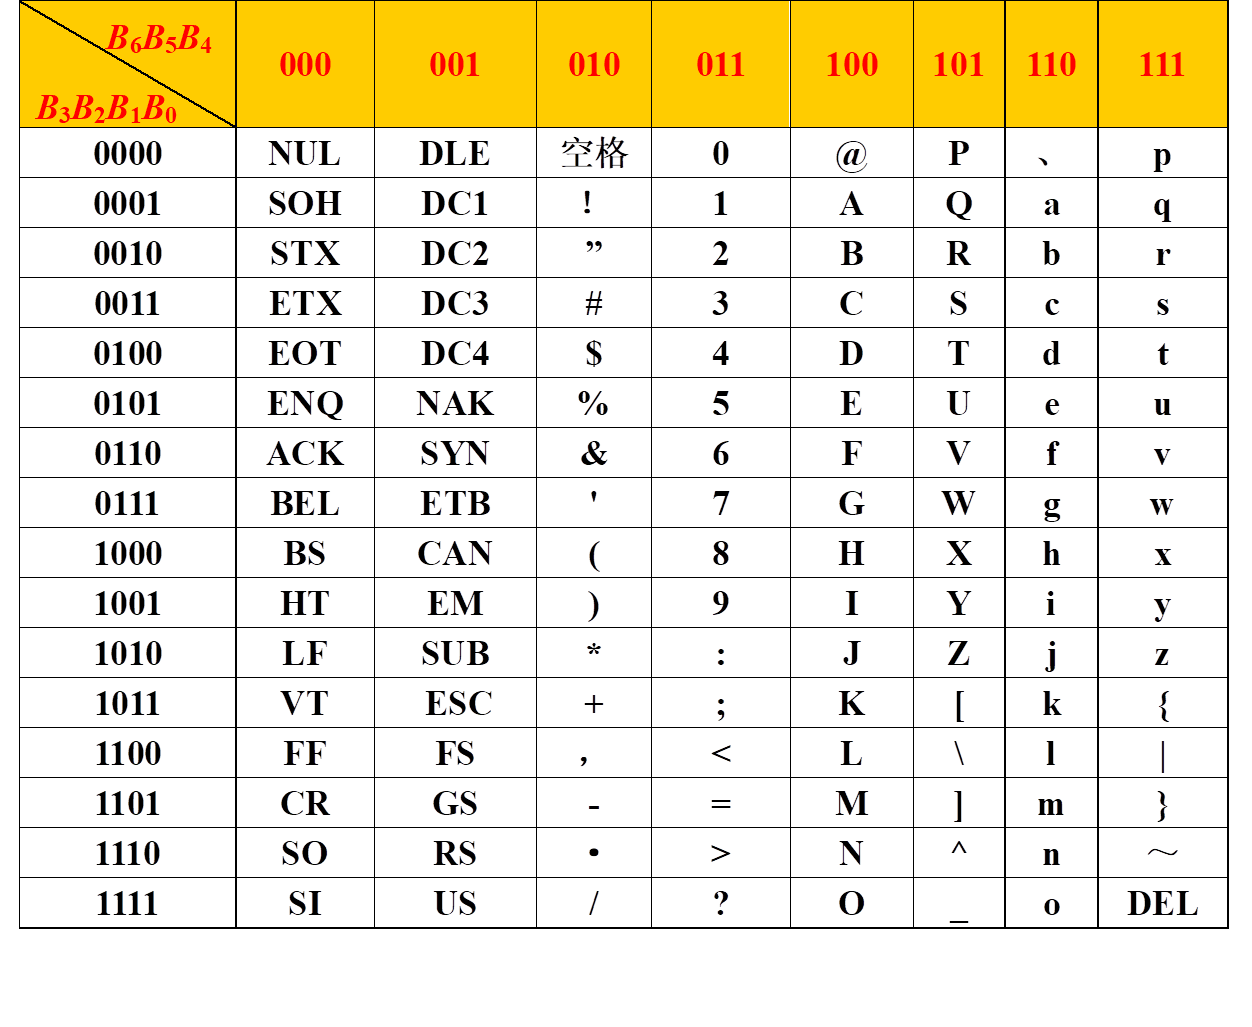
\includegraphics[scale=0.4]{ASCII}
	\column{0.35\textwidth}
	\begin{itemize}
		\item ASCII码连续排列 \\
		`0'$\sim$`9', `A'$\sim$`Z', `a'$\sim$`z'
		\item 数字 = 编码值 - `0' \\
		9=`9'-`0'
		\item 大小字符间隔: \\
		`a' - `A' = 32
		
		\scriptsize{
			`a'=0110~0001=61H=0X61=97
			
			'A'=0100~0001=41H=0X41=65}
	\end{itemize}	
\end{columns}
\end{frame}

\begin{frame}[shrink,fragile]{字符类型}
\begin{lstlisting}
#include<stdio.h>           
int main()                   
{                            
	char c1 = 'A', c2 = 'a', c3 = '\n'; // 字符型变量, 
	// '\n': 表示特殊字符 --- 换行符
	printf("%c,%c,%d\n",c1,c2,c3); // A,a,10
	// 整型变量的整数值就是ASCII编码值
	printf("%c,0X%x,%d\n",c1,c1,c1); // A,0X41,65
	c1 = c1 + 1; // 在表达式中, char类型当作int处理
	printf("%c,0X%x,%d\n",c1,c1,c1); // B,0X42,66
	c1 = c1 + 32;  // 转换为小写字母
	printf("%c,0X%x,%d\n",c1,c1,c1); // b,0X62,98
	printf("%d\n",'9'-'0'); // 数字 = 编码值- '0'
	printf("%c,%d,%c,%d\n",'A','A','a','a'); // 输出字符和相应的ASIII编码
	return 0;           
}                            
\end{lstlisting}
\end{frame}


\begin{frame}[shrink,fragile]{常量}
\vspace{-0.2cm}
\begin{lstlisting}
#include<stdio.h> 
#define PI 3.14  // 符号常量, 注意没有分号           
int main()                   
{                                  
	int a = 123; // 整型常量
	float f = 12.2, f1=123E-1; // 实型常量, $123\times 10^{-1}$
	char c1 = 'A', c2='\n'; // 字符常量, 特殊字符 --- 换行符
	char s[50] = "boy"; // 字符串常量
	printf("半径为%d的圆周长是%f\n",a,2*PI*a);       
	printf("回车换行\n");
	printf("单引号\',双引号\"转义字符前缀\,\n");  
	return 0;           
}                            
\end{lstlisting}
\textcolor{blue}{转义字符(特殊字符), 见p40, 表3.1}
\end{frame}

\begin{frame}[fragile]{常量与常变量}
\begin{lstlisting}
#include<stdio.h> 
#define PI 3.14  // 符号常量, 注意没有分号           
int main()                   
{                            
	int r = 123; // 整型变量
	const int a = 425; // 常变量
	r = 100; // 合法, 因为r是变量,可以随时更改它的值
	a = 100; // 不合法,因为a是常变量,不能更改
	printf("半径为%d的圆周长是%f\n",r,2*PI*r); 
	return 0;           
}                            
\end{lstlisting}
\end{frame}

\begin{frame}[fragile,shrink]{长整型、无符号整型, 浮点型数据类型}
\begin{lstlisting}
#include<stdio.h>           
int main()                   
{                            
	int a = 123; // 整型变量
	long int b = 1E+8; // 长整型变量
	unsigned int u = 0XFF; // 无符号整型, 最高位不作为符号位处理
	float f = 10.2; // 单精度浮点数
	double d = 1E-8; // 双精度浮点数
	printf("%x,%d\n",u,u); // ff, 255
	printf("%d,%ld,%x,%f,%lf\n",a,b,u,f,d);
	// sizeof函数返回类型分配的字节数,整型数据存储空间和值的范围见p45, 表3.2
	printf("%d,%d,%d,%d\n",sizeof(int),sizeof(float),sizeof(double),sizeof(long int),sizeof(long long int));
	return 0;           
}                            
\end{lstlisting}
\end{frame}




%%%%%%%%%%%%%%%%%%%%%%%%%%% lecture-3
%\begin{frame}
%  \frametitle{lecture-3 主要内容}
%  \framesubtitle{最简单的C语言程序设计---顺序程序设计}
%  \tableofcontents[hideallsubsections]
%\end{frame}

\section{数据的输入输出}

\begin{frame}{常用格式描述符与数据类型的对应关系}
\begin{tabular}{|c|c|c|}
	\hline 
	\textbf{格式符} & \textbf{对应的数据类型} &  \textbf{备注}\\ 
	\hline 
	\%d & int &  \\ 
	\hline  
	\%f & float &  \\
	\hline
	\%c & char & \\ 
	\hline   
	\%lf & double & \\ 
	\hline 
	\%.2f & float & 保留两位小数, 四舍五入。不适用于scanf()。 \\ 
	\hline 
	\%.2lf & double & 保留两位小数, 四舍五入。不适用于scanf()。 \\ 
	\hline
	\hline   
	\%x & int & 十六进制显示 \\ 
	\hline 
	\%ld & long int &  \\ 
	\hline 
\end{tabular}
\newline
\newline
\textcolor{blue}{详见p73, 表3.6}
\end{frame}

\begin{frame}[shrink,fragile]{输出语句printf(``原样输出, \%格式符'', 对应变量值);}
\begin{lstlisting}
#include<stdio.h>            // standard input/output编译预处理指令
int main()                   // 主函数
{                            // 函数开始标志
   int a=10,b;    // 定义变量a, b为整型数值, 定义变量时,可以指定变量的初值
   float f=10.2;  // 定义变量f为单精度浮点数
   double d; // 定义变量d为双精度浮点数
   char c;   // 定义变量c为单个英文字母
   f=10.2;
   d=20.356;
   c='A';
   printf("a=%d,b=%d,c=%c,f=%f,d=%.2lf\n",a,b,c,f,d); // %.2f, %.2lf保留两位小数
   return 0;                 // 函数执行完毕返回函数值0
}                            // 函数结束标志
\end{lstlisting}
\textcolor{blue}{变量b没有被赋值, 将是一个随机值。}
\end{frame}

\begin{frame}[fragile]{输入语句scanf(``\%变量格式符'', \&变量名);}
\begin{lstlisting}
#include<stdio.h>            // standard input/output编译预处理指令
int main()                   // 主函数
{                            // 函数开始标志
   int a=10,b;    // 定义变量a, b为整型数值, 定义变量时,可以指定变量的初值
   float f=10.2;  // 定义变量f为单精度浮点数
   double d; // 定义变量d为双精度浮点数
   char c='A';   // 定义变量c为单个英文字母, 字符输入以后讲
   printf("请输入整数和浮点数, 空格隔开:\n"); // 提示语句[可选]
   scanf("%d%f",&a,&f);  // 尽量简单, 不要有其它字符和'\n'
   printf("请输入两个浮点数, 空格隔开:\n"); // 提示语句[可选]
   scanf("%f%lf",&f,&d);
   printf("a=%d,b=%d,c=%c,f=%f,d=%lf\n",a,b,c,f,d); // \n为换行符
   return 0;                 // 函数执行完毕返回函数值0
}                            // 函数结束标志
\end{lstlisting}
\end{frame}

\begin{frame}[fragile]{字符输出函数putchar}
\begin{lstlisting}
#include<stdio.h>
int main()
{
   char a = 'B',b = 'O',c = 'Y'; //定义3个字符变量并初始化
   putchar(a); //向显示器输出字符B
   putchar(b); //向显示器输出字符O
   putchar(c); //向显示器输出字符Y
   putchar ('\n'); //向显示器输出一个换行符
   return 0;
}
\end{lstlisting}
\end{frame}

\begin{frame}[fragile]{字符输入函数getchar, 遇到回车, 开始从缓冲区中接收字符。}
\vspace{-0.4cm}
\begin{lstlisting}
#include<stdio.h>
int main()
{
   char a,b,c;  //定义字符变量a,b,c
   a = getchar();  //从键盘输入一个字符,送给字符变量a
   b = getchar();  //从键盘输入一个字符,送给字符变量b
   c = getchar();  //从键盘输入一个字符,送给字符变量c
   putchar(a);  //将变量a的值输出
   putchar(b);  //将变量b的值输出 
   putchar(c);  //将变量c的值输出
   printf("\na=%d,b=%d,c=%d,a=%c,b=%c,c=%c\n",a,b,c,a,b,c);
   return 0;
}
\end{lstlisting}
\end{frame}

\begin{frame}[fragile]{\small 字符输入函数getchar, 遇到回车, 开始从缓冲区中接收字符。}
\begin{lstlisting}
char a,b,c;  //定义字符变量a,b,c
a = getchar();  //从键盘输入一个字符,送给字符变量a
b = getchar();  //从键盘输入一个字符,送给字符变量b
c = getchar();  //从键盘输入一个字符,送给字符变量c
putchar(a);  //将变量a的值输出
putchar(b);  //将变量b的值输出 
putchar(c);  //将变量c的值输出
printf("\na=%d,b=%d,c=%d,a=%c,b=%c,c=%c\n",a,b,c,a,b,c);
\end{lstlisting}
从键盘输入abc回车, 观察结果, 应该是正确的结果。
遇到回车, 开始从缓冲区中接收字符。
\end{frame}

\begin{frame}[fragile]{\small 字符输入函数getchar, 遇到回车, 开始从缓冲区中接收字符。}
\begin{lstlisting}
a = getchar();  //从键盘输入一个字符,送给字符变量a='a'
b = getchar();  //从键盘输入一个字符,送给字符变量b='\n'
c = getchar();  //从键盘输入一个字符,送给字符变量c='b'
putchar(a);  //将变量a的值输出a
putchar(b);  //将变量b的值输出\n 
putchar(c);  //将变量c的值输出b
printf("\na=%d,b=%d,c=%d,a=%c,b=%c,c=%c\n",a,b,c,a,b,c);
\end{lstlisting}
再运行一次程序, 输入a回车, 输入b回车, 输入c回车, 观察结果。\\
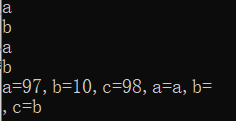
\includegraphics[scale=0.5]{abc}
\end{frame}

\begin{frame}{开发平台上演示讲解}
在开发平台,以具体的示例,详细讲解以下内容:
\begin{itemize}
	\item int, float, double, char 数据类型, sizeof(~)函数
	\item \%d, \%f, \%c, \%lf, \%x格式符的使用(见ppt中的表格)
	\item if(~)\{\quad\}, while(~)\{\quad\}简单语句
	\item char c; scanf(``\%c", \&c); 接收输入的字符
	\item char c; c=getchar()接收输入的字符, putchar()输出一个字符
	\item 编程理解数字ASCII码与整数的对应关系以及大小写字符之间的关系。
	\item 避免数字,字符在一条语句中输入的情况,如:\\ scanf(``\%d\%c\%d",...);
	\item 重点理解字符缓冲区的概念,以及消费无用字符的技巧。
\end{itemize}
\end{frame}

\note
{
根据学生的反馈,数据的输入语句没有完全听明白。 \\
下一讲, 进一步详细讲解。\\
欢迎同学们在群里踊跃发言,任何不理解的知识点请指出来,我将在以后的讲课中,有针对性的讲清楚大家有疑惑的问题。一些与编程无关的俏皮话之类的东西就不要发了,争取把我们这个群建立成纯净的,对大家学习课程有帮助的程序设计讨论群。力争100名学生一个都不掉队,考个好成绩。加油!!
}





%%%%%%%%%%%%%%%%%%% last frame
\begin{frame}[plain]{}
  \begin{center}
    \begin{tikzpicture}
      \node[above,xscale=1.2,yscale=1.2]{\Huge 欢迎批评指正!};
    \end{tikzpicture}
  \end{center}
\end{frame}

\end{document}


%%%%下面的内容不参与文档的编译。使用者在想用某个东西时直接可通过查阅,并复制黏贴和修改使用。

\iffalse  %注释开始

\section{第一部分}

%垂直居中
\begin{frame}
  \begin{center}
  需要居中的内容!
  \end{center}
\end{frame}
或者
\begin{frame}
  \centering
  一些内容
\end{frame}

%幻灯片标题的使用
\begin{frame}
\frametitle{第一部分第一张幻灯}
  一些内容
\end{frame}

%项目编号的使用
\begin{frame}
  \frametitle{条目}
  \begin{itemize}
  \item 项目1
  \item 项目2
  \item 项目3
  \item 项目4
    \begin{itemize}
    \item 二级项目1
    \item 二级项目2
    \end{itemize}
  \end{itemize}
\end{frame}

%表格的使用
\begin{frame}
  \frametitle{表格}
  \begin{table}[htbp!]
  	\small %\tiny,\scriptsize,\footnotesize,\small,\normalsize,\large,\LARGE,\huge,\Huge
    \centering
    \caption{主流机器学习框架}
    \begin{tabular}{c|c|c|c|c}
      \toprule[1pt]
      机器学习库	& 机构 & 支持语言  & 平台 & Tensor \\
      \toprule[1pt]
      TensorFlow	& Google & C++,Python &跨平台 & Good \\
 	  \hline
      Pytorch	&  Facebook& Python & 跨平台 & Good \\
 	  \bottomrule[1pt]
    \end{tabular}
  \end{table}
\end{frame}

%区块的使用
\begin{frame}
  \frametitle{分析}
  \begin{block}{XXX 算法}
	\begin{itemize}
		\item 步骤1
	 	\item 步骤2
	 	\item 步骤3
	 \end{itemize}
  \end{block}
\end{frame}

%使用区块来强调内容
\begin{frame}
  \frametitle{强调}
  \begin{itemize}
  \item 这是内容
  \end{itemize}
  \only<1>\begin{block}{}
    这里蹦出来一个强调!
  \end{block}
\end{frame}

%section中目录的使用
\begin{frame}
  \frametitle{技术影响力}
    \tableofcontents[currentsection,hideallsubsections]
\end{frame}

%插入图片
\begin{frame}
\begin{figure}[!h]
  \centering
  % Requires \usepackage{graphicx}
  \includegraphics[width=2cm]{pics/logo.jpg}\\
  \caption{logo图片样例}\label{pic6}
\end{figure}
\end{frame}

%分栏实现图文混排
\begin{frame}
分栏前面的一些内容!!
\begin{columns}%0.6 0.4表示相对比例
\column{0.6\textwidth}%<1->
分栏的左侧,文字叙述。
\column{0.4\textwidth}%<1->
分栏的右侧插入了图片。
 \begin{figure}[!h]
  \centering
  % Requires \usepackage{graphicx}
  \includegraphics[width=4cm]{pics/logo.jpg}\\
  \caption{logo图片样例}\label{pic6}
\end{figure}
\end{columns}
分栏后面的一些内容!!
\end{frame}

%% last frame
\begin{frame}[plain]{}
\begin{center}
	\begin{tikzpicture}
	\node[above,xscale=1.2,yscale=1.2]{\Huge 欢迎批评指正!};
	\end{tikzpicture}
\end{center}
\end{frame}

% 大括号
$\left\{ .....  \right\}$
$\left[ .....  \right]$
$\left( ..... \right)$
$\left\{ .....  \right.$ %有左无右

$\delta_{jk}=
\begin{cases}
1, & (i=k)\\
0, & (i\ne k)
\end{cases}
$

\tikzstyle{int}=[draw, fill=blue!20, minimum size=2em]
\tikzstyle{init} = [pin edge={to-,thin,black}]
\begin{tikzpicture}[node distance=2.5cm,auto,>=latex']
\node [int, pin={[init]above:$v_0$}] (a) {$\frac{1}{s}$};
\node (b) [left of=a,node distance=2cm, coordinate] {a};
\node [int, pin={[init]above:$p_0$}] (c) [right of=a] {$\frac{1}{s}$};
\node [coordinate] (end) [right of=c, node distance=2cm]{};
\path[->] (b) edge node {$a$} (a);
\path[->] (a) edge node {$v$} (c);
\draw[->] (c) edge node {$p$} (end) ;
\end{tikzpicture}

%%%%%%%%%% 上下文字
$P(H_1|H_0)\mathop{=}\limits^{def}P_F$\\    %上下文字在\[... \]和$...$表现不一致
\[P(H_1|H_0)\mathop{=}\limits^{def}P_F \]
\[P(H_1|H_0)\mathop{=}^{def}P_F \]
\begin{align*}
P(H_1|H_0)\mathop{=}^{def}P_F
\end{align*}

\begin{enumerate}
	\setcounter{enumi}{3} %设定起始编号 
	\item aaa
	\item bbb
\end{enumerate}

%%%%%%%%%%%
\\
~\\ %一行空白

\newline
\newline
%%%%%%%%%%%%

\bigskip  或\medskip

%%%%%%%%%%%%%%%% 自动压缩,以显示全部内容
\begin{frame}[shrink]
\frametitle{标题} %需要页面标题时,这样设置,而不能\begin{frame}{标题}[shrink]
\end{frame}

%%%%%%%%%%%% 最后一列左对齐---&&, 单个&分割,则是右对齐
\begin{align*}
E[a(t)]&=\int_{-\infty}^{\infty}a(t)p(x)dx\\
&=a(t)\int_{-\infty}^{\infty}p(x)dx &&\text{by $a(t)$是常数}\\
&=a(t)\cdot 1 &&by \int_{-\infty}^{\infty}p(x)dx=1\\
&=a(t)
\end{align*}

%%%%%%%%%%%%%%%%有色文本
\textcolor{blue}{This text is in blue} 
\colorbox{yellow}{This text is highlighted in yellow} 
\colorbox{yellow}{ 
	\textcolor{red}{ 
		\textbf{ 
			Bold text in red, highlighted in yellow 
		} 
	} 
} 

block 普通环境
theorem 定理环境
lemma 引理环境
proof 证明环境
corollary 推论环境
example 示例环境
alertblock 警示环境

\begin{frame}{算法}
\begin{columns}[T] % align columns
	\begin{column}<0->{.5\textwidth}
		\begin{algorithm}[H]  
			\caption{algorithm caption} %算法的名字
			\hspace*{0.02in} {\bf Input:} %算法的输入, \hspace*{0.02in}用来控制位置,同时利用 \\ 进行换行
			input parameters A, B, C\\
			\hspace*{0.02in} {\bf Output:} %算法的结果输出
			output result 
			\begin{algorithmic}[1] %每行显示行号  
				\State some description % \State 后写一般语句
				\For{condition} % For 语句,需要和EndFor对应
				\State ...
				\If{condition} % If 语句,需要和EndIf对应
				\Else
				\EndIf
				\EndFor
				\While{condition} % While语句,需要和EndWhile对应
				\EndWhile
				\State \Return result	
			\end{algorithmic}  
		\end{algorithm}
	\end{column}%
	\hfill%	
	\begin{column}<0->{.40\textwidth}
		
	\end{column}%
\end{columns}
\end{frame}

\begin{frame}[fragile]{代码}
\fontspec{Consolas}
%不能用Tab键
\begin{lstlisting}
inline int gcd(int a, int b) { 
return b==0?a:gcd(b,a%b)
}
inline int lcm(int a, int b) {
return a/gcd(a,b)*b;
}
\end{lstlisting}
\end{frame}

\fi   %注释结束
